\section{Лекция 7. Лемма Гурса. ИТК}
\subsection{Лемма Гурса}
\textbfit{Лемма Гурса.} Пусть $f: \mathbb{C} \to \mathbb{C},\  D \ -$ область, $f \in \mathcal{O}(D)$. Тогда $\forall$ треугольника $\Delta$, т.ч. замыкание $\overline{\Delta} \subset D \ \int_{\partial \Delta}f(z) dz = 0$.
\[\triangleright \text{ От противного. Пусть } \exists \Delta_0 : \left|\int_{\partial \Delta_0} f(z) dz\right| = M > 0\]

\begin{minipage}{0.25\textwidth}
    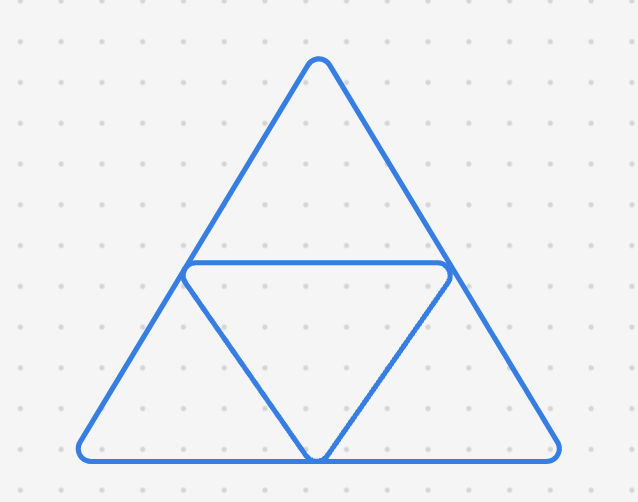
\includegraphics[width=\textwidth]{lection7_1.png}
\end{minipage}
\begin{minipage}{0.65\textwidth}
    \[\text{Разобьём его на 4 $\triangle$ средними линиями и выберем $\Delta_1 :$}\] 
    \[\left|\int_{\partial \Delta_1} f(z) dz\right| \geq \frac{M}{4}\]
    \[\overline{\Delta_0} \supset \overline{\Delta_1} \supset \ldots \supset \overline{\Delta_n} \supset \ldots, \ \left|\int_{\partial \Delta_n} f(z) dz \right| \geq \frac{M}{4^n}\]
\end{minipage}
\[\Rightarrow \exists ! z_0 = \bigcap_{i}^\infty \overline{\Delta_n}, \ z_0 \in D \Rightarrow f \text{ голоморфна в }z_0\]
\[\Rightarrow \forall \epsilon > 0 \ \exists \delta(\epsilon) > 0 : \ \forall z \in U_\delta (z_0) \subset D\]
\[f(z) = f(z_0) + f'(z_0)(z-z_0) + \alpha(z)(z-z_0), \ |\alpha(z)| < \epsilon\]
\[\exists n : \ \Delta_n \subset U_\delta(z)\]
\[\frac{M}{4^n} \leq \left|\int_{\partial \Delta_n} d(z) dz\right| = \left|\int_{\partial \Delta_n} f(z_0) dz + \int_{\partial \Delta_n} f'(z_0)(z-z_0) dz + \int_{\partial \Delta_n} \alpha(z)(z-z_0)dz\right| =\]
\[= \left| \begin{array}{ll}
    \int_\Gamma z^n dz = \frac{\Gamma^{n+1}(b) - \Gamma^{n+1}(a)}{n+1} \\
    n \neq -1
\end{array}\right| = \left|\int_{\partial \Delta_n} \alpha(z)(z-z_0)dz\right| < \epsilon \left| \text{диаметр } \triangle \right| \cdot |\partial \triangle_n|  < \epsilon \cdot |\partial \Delta_n|^2  =\] 
\[= \epsilon \left(\frac{|\partial \Delta_0|}{2^n}\right)^2 = \frac{\epsilon |\partial \Delta_0|^2}{4^n}\]
\[M < \epsilon |\partial \Delta_0|^2 \ \forall \epsilon > 0 \Rightarrow M = 0 \text{ противоречие } \blacktriangleleft\]

\textbfit{Сл.} $\forall$ многоугольника это тоже верно.

\textbfit{Теорема.} Пусть $D \subset \mathbb{C}, D \ -$ область, $f:D \to \mathbb{C}, f \in C(D), \ \gamma \ -$ кусочно-гладкая кривая в $D$. Тогда $\forall \epsilon > 0 \ \exists L \subset D \ - $ ломаная, т.ч. $\left|\int_\gamma f(z) dz - \int_L f(z) dz\right| < \epsilon$.
\[\triangleright \ 1) \ \exists \text { ограниченная область $D_1$, т.ч. } \overline{D_1} \subset D, \ \gamma \subset D_1.\]
\[\forall z \in \gamma \ \exists U_{\delta(z)}(z) \subset D.\] 
\[\text{Рассмотрим } \left\{U_{\frac{\delta(z)}{2}}(z)\right\} \text{ -- покрытие $\gamma$, выберем конечное подпокрытие } \left\{U_{\frac{\delta(z_n)}{2}}(z_n)\right\}_{n=1}^N.\]
\[\text{Положим } D_1 := \bigcup_1^N U_{\frac{\delta(z_n)}{2}}(z_n) \Rightarrow \overline{D_1} \subset D, \gamma \in D_1\]
\[dist (\gamma, \partial D_1) = d > 0\]
\[\text{Тогда будем выбирать разбиение $[a;b]$, по которому пробегает $\gamma$, $z_k = \Gamma(t_k) : |z_{k-1} z_k| < d$.} \]
\[\gamma_k = \Gamma([t_{k-1}, t_k])\]
\[|\gamma_k| = \int_{t_{k-1}}^{t_k} |\dot{\Gamma}(t)| dt \leq M |t_k-t_{k-1}|\]
\[\text{Тогда } L = z_0z_1\ldots z_n \subset D_1\]
\[\overline{D_1} \text{ -- компакт, } \overline{D_1} \subset D \Rightarrow f \in C(\overline{D_1}) \Rightarrow \text{равномерно непрерывная} \Rightarrow\]
\[\Rightarrow \forall \epsilon > 0 \ \exists \delta_1(\epsilon): \ \forall z_1, z_2 : |z_1-z_2| < \delta_1 \Rightarrow |f(z_1)-f(z_2)| < \frac{\epsilon}{|\gamma|}\]
\[\text{Тогда берём разбиение $[a; b]$ т.ч. $|z_{k-1}z_k| < \min(d, \delta_1)$.}\]
\[\left|\int_\Gamma f(z) dz - \int_L f(z) dz\right| = \left|\sum \int_{\Gamma_k}f(z) dz - \sum \int_{[z_{k-1},z_k]}f(z)dz\right| = \left|\sum_{k=1}^n \left(\int_{\Gamma_k}f(z) dz -\right.\right.\] 
\[- \left.\left.\int_{\Gamma_k}f(z_{k-1}) dz \right) + \sum_{k=1}^n \left(\int_{\Gamma_k}f(z_{k-1}) dz - \int_{[z_{k-1},z_k]}f(z) dz\right)\right| =\] 
\[= \left|\int_{\Gamma_k} f(z_{k-1})dz =\int_{[z_{k-1}, z_k]} f(z_{k-1})dz_k \right| \leq \frac{\epsilon}{|\gamma|} \sum_1^n |\Gamma_k| + \sum \left|\int_{[z_{k-1}, z_k]}(f(z_{k-1}) - f(z))dz\right| \leq\]
\[\leq \epsilon + \frac{\epsilon}{|\gamma|} \sum_1^n |z_{k-1}z_k| < \left|\sum_1^n |z_{k-1}z_k| = |L| < |\gamma|\right| < 2\epsilon \ \blacktriangleleft\]

\textbfit{Сл.} (б/д) Пусть $f:\overline{D} \to \mathbb{C}, \partial D \ - $ кусочно-гладкая жорданова замкнутая кривая, $D \ -$ ограниченная область, $f \in C(\overline{D})$. Тогда $\forall \epsilon > 0 \ \exists L \ -$ замкнутая ломаная $L \subset D:$ 

$\left|\int_{\partial D} f(z) dz - \int_L f(z) dz\right| < \epsilon$.

\textit{Отличие от предыдущей теоремы}: в предыдущей теореме наша ломаная может выходить наружу области; эта же теорема говорит, что обязательно сможем построить ломаную, которая полностью лежит внутри области.

\textbfit{Опр.} Область в $\mathbb{C} (\overline{\mathbb{C}})$ называется односвязной, если её граница в $\overline{\mathbb{C}}$ состоит из 0 точек, 1й точки или 1й жордановой кривой (возможно, несобственной).

\subsection{ИТК}
\textbfit{Теорема} (Интегральная теорема Коши для односвязных областей). Пусть $f:D \to \mathbb{C}, f \in \mathcal{O}(D), \overline{G} \subset D, G \ - $ ограниченная односвязная область, $\partial G \ -$ кусочно-гладкая замкнутая жорданова кривая. Тогда $\int_{\partial G} f(z) dz = 0$.
\[\triangleright \text{ По следствию } \forall \epsilon > 0 \ \exists L \subset G \text{ -- замкнутая т.ч. } \left|\int_{\partial G} f dz - \int_L fdz\right| < \epsilon\]
\[\Rightarrow L \text{ -- граница многоугольника } M, \overline{M} \subset G \text{, т.к. $G$ -- односвязная}\]
\[\Rightarrow \text{ по сл. из л. Гурса } \int_L f(z) dz = 0 \Rightarrow \left|\int_{\partial G} f(z) dz\right| < \epsilon \ \forall \epsilon > 0 \Rightarrow \int_{\partial G} f(z) dz = 0 \blacktriangleleft\]

\textbfit{Теорема} (ИТК для многосвязных областей) (б/д). Пусть $f:D\to \mathbb{C}, \overline{G} \subset D, G \ -$ ограниченная область, $\partial G$ состоит из конечного числа замкнутых непересекающихся кусочно-гладких жордановых кривых. Тогда $\int_{\partial G^+} f(z) dz = 0$.
